\documentclass[12pt]{article}

\input ElvisMacros.mac
%\usepackage{showkeys}
\usepackage{array}
\usepackage{pgfplots}


\begin{document}

\setcounter{section}{4}
\setcounter{figure}{0
}


\begin{center}
{\LARGE\bf\underline{Notes on the Elvis Problem, Part II}}
\end{center}


\section{Minimal time functions}\label{sec: min time}
A minimal time problem uses the data of a controlled dynamical system and a target set.  The problem consists of finding the fastest way to go from a given initial point to some point on the target by following a trajectory of the dynamical system.  An optimal trajectory is one that achieves this aim.  The Elvis problem has velocity sets that are fixed (that is, they do not depend on an individual point in a region, but only on the region itself.  As such, an optimal trajectory, while it remains in a region, will use only one velocity, and is therefore a straight line.  This allows for a considerable simplification of the analysis, and allows for the concepts introduced in Part I to be used instead of a more general and complicated dynamical systems theory.   

\subsection{One region with Constant Dynamics}
We first consider the case where the velocity set is the same throughout $\R^n$.  Let $F\in\cC$.  

\begin{defn}
A trajectory of $F$ is a piece-wise differentiable function $x(\cdot):[0,T]\to\R^n$ with $\dot x(t)\in F$.
For $X\in\R^n$ and $T>0$, the Reachable Set from $X$ at time $T$ is defined by 
\[
R^{(T)}(X):=\bigl\{x(T):\;x(\cdot)\text{ is a trajectory of } F\bigr\}.
\]
\end{defn}

{\blue
\begin{exer}  Let $X_1\in\R^n$ and $T>0$.
\begin{itemize}
\item[(a)]  Show that $R^{(T)}(X_1)=X_1+TF:=\bigl\{X_1+Tv:\;v\in F\bigr\}$.
\item[(b)]  Characterize those $X_2\in\R^n$ for which $X_2\in R^{(T)}(X_1)$ for some $T>0$. 
\item[(c)]  Show that
\[
\gamma_F\left(X_2-X_1\right)=\inf\biggl\{T:\;\exists \text{ trajectory }x(\cdot)\text{ of }F\text{ with }x(0)=X_1,\,x(T)=X_2\biggr\}
\]
(Recall $\inf\emptyset=+\infty$.)
\item[(d]  Let $\bd v:=\frac{X_2-X_1}{\gamma_F(X_2-X_1)}\ed$ and $T:=\gamma_F(X_2-X_1)$.  Show that the optimal trajectory from $X_1$ to $X_2$ is given by $x(t)=X_1+ t v$ for $t\in[0,T]$.
\end{itemize}
\end{exer}
}

Suppose $S\subseteq\R^n$ is any closed set (the \lq\lq target\rq\rq) and $F\in\cC$ (the \lq\lq admissible velocities\rq\rq).  The so-called minimal time function $T_S(\cdot)$ determined by $S$ and
$F$ is defined by
\[
T_S(x)=\min\biggl\{t:[x+tF]\cap S \not= \emptyset\biggr\}.
\]

{\blue
\begin{exer}
Show that $T_{S}(x)=\inf\bigl\{T:R^{(T)}(X)\cap S\not=\emptyset\bigr\}=\inf\bigl\{\gamma_{F}(y-x):\;y\in S\bigr\}$.
\end{exer}
}

\subsection{Two regions with different velocity sets}
Of course our Elvis problem does not have one single velocity set on the whole space, but rather different velocity sets on different regions with an interface separating the regions.  We eventually will want more general configurations, but for now we begin with only two open half spaces $\cM_1$ and $\cM_2$.  In this case there is a vector $\vec n\not=\0$ and a number $r\in\R$ so that 
\[
\cM_1=\bigl\{x:\;\langle\vec n,x\rangle < r\bigr\}\quad\text{and}\quad
\cM_2=\bigl\{x:\;\langle\vec n,x\rangle > r\bigr\},
\]
and the interface is 
\[
\Sigma:=\bdry(\cM_1)\cap \bdry(\cM_2)=\bigl\{x:\;\langle\vec n,x\rangle = r\bigr\}.
\]
Each $\cM_i$, $i=1,2$, has an associated velocity set $F_i\in\cC$.  First, consider the case where $X_1\in\cM_1$ and $X_2\in\cM_2$, and we want to travel from $X_1$ to $X_2$ in the least time.  We elaborate on what we mean by \lq\lq travel.\rq\rq\ Any function $x(\cdot):[0,T]\to\R^n$ that is differentiable at every $t\in[0,T]$ except possibly finite many points $\{t_1,\,t_2,\dots,\,t_m\}$ is called an {\it arc}.  If an arc $x(\cdot)$ satisfies
\[
x(t)\in \cM_i,\,t\in[0,T]\backslash\{t_1,\,t_2,\dots,\,t_m\}\quad\Longrightarrow\quad
\dot x(t)\in F_i,
\]  
then $x(\cdot)$ is called a trajectory (of the system).  Thus \lq\lq to travel from $X_1$ to $X_2$ in the least time\rq\rq\ means to find a trajectory that satisfies $x(0)=X_1$, $x(T)=X_2$, and where $T$ is as small as possible.
Formally, the {\it minimal time problem} is stated as
\begin{equation}\label{eq: Elvis1}\tag{$\cP1$}
\min\; T\qquad\text{such that }\exists\text{ trajectory }x(\cdot):[0,T]\to\R^n\text{ with }x(0)=X_1, x(T)=X_2.
\end{equation} 
The reachable set $R^{(T)}(X_1)$ is defined as before in that it consists of all points $X_2$ for which there exists a trajectory $x(\cdot)$ for which $x(0)=X_1$ and $x(T)=X_2$.

{\blue
\begin{exer}\label{exer: 1}  This exercise refers to ($\cP1$) where $X_1\in\cM_1$ and $X_2\in\cM_2$.
\begin{itemize} 
\item[(a)]  Show an optimal trajectory which begins at $X_1\in\cM_1$ will leave $\cM_1$ and not return to any point in $\cM_1$.
\item[(b)]  Show that ($\cP1$) is equivalent to
\begin{equation*}\label{eq: prob}
\min\;\biggl\{\gamma_1(Q-X_1)+\gamma_2(X_2-Q)\biggr\}\quad\text{over}\;Q\in\Sigma
\end{equation*}
\item[(c)]  Deduce that ($\cP1$) is equivalent to
\begin{equation*}\tag*{\begin{color}{black}($\cP2$)\end{color}}
\min\;\biggl\{\gamma_1(Q-X_1)+\gamma_2(X_2-Q)+\cI_{\Sigma}(Q)\biggr\}\quad\text{over }Q\in\R^n
\end{equation*}
\end{itemize}
(Two problems are \lq\lq equivalent\rq\rq\ if a solution of one can lead to a solution of the other.)
\end{exer}
}

We now introduce a further assumption.
\begin{align}\tag{H1}
\text{Each }F_i \text{ belongs to }\cC_0.
\end{align}
One of the consequences of this assumption is that for every $X_1,\,X_2\in\R^n$, the problem ($\cP1$) has a feasible solution.  This is because there are \lq\lq admissible\rq\rq\ velocities in every direction, and thus there is at least one trajectory $x(\cdot)$ defined on some interval $[0,T]$ with $x(0)=X_1$ and $x(T)=X_2$.  

{\blue
\begin{exer}  Assume (H1) holds.
\begin{itemize}  
\item[(a)]  For every $X_1,\,X_2\in\R^n$, show there is at least one trajectory $x(\cdot)$ from $X_1$ to $X_2$ (consider different cases on whether the $X_i$'s belong to the same half space).
\item[(b)]  What are the necessary conditions for a trajectory $x(\cdot)$ to solve ($\cP1$)?
\item[(c)]  Assuming  $X_1\in\cM_1$ and $X_2\in\cM_2$, what are the necessary and sufficient conditions for a point $Q\in\R^n$ to solve ($\cP2$)?
\end{itemize}
\end{exer}}

Part (b) of the last exercise is a trick question, for it depends on whether $X_1$ and $X_2$ belong to the same manifold or not.  Let us first assume $X_1\in\cM_1$ and $X_2\in\cM_2$ as in part (c), in which case we can rely on the results in Exercise~\ref{exer: 1}.  Indeed, via Rockafellar's Theorem, there exists $Q\in\Sigma$ and two vectors $\zeta_1,\,\zeta_2\in\R^n$ satisfying
\begin{eqnarray}
\zeta_1&\in &\partial\gamma_{F_1}(Q-X_1),  \label{eq: zeta1}\\
 -\zeta_2&\in &\partial\gamma_{F_2}(X_2-Q),\quad\text{and}  \label{eq: zeta2}\\
\zeta_1-\zeta_2 &\in & N_{\Sigma}(Q).  \label{eq: normal}
\end{eqnarray}
Using Exercise~4.2, we have for each $i=1,\,2$ that
\begin{equation}\label{eq: polar = 1}
\gamma_{F_i^{\circ}}(\zeta_i)=1 .
\end{equation}
We know $\bd v_1:=\frac{Q-X_1}{\gamma_{F_1}(Q-X_1)}\in F_1\ed$ and $\bd v_2=\frac{X_2-Q}{\gamma_{F_2}(X_2-Q)}\in F_2\ed$ are the two velocities used by the optimal trajectory, and by Exercise~4.2 again, that
\begin{align}
v\mapsto \langle\zeta_1,v\rangle\quad &\text{is maximized over }v\in F_1\text{ at } v=v_1 \label{eq: MP1}\\
v\mapsto \langle-\zeta_2,v\rangle\quad &\text{is maximized over }v\in F_2\text{ at } v=v_2. \label{eq: MP2}
\end{align}

\begin{Exam}\label{Snell's Law}{\rm
Let us now specialize to the case $n=2$, $\cM_1$ (resp. $\cM_2$) the upper (resp. lower) half-plane, $\Sigma$ the $x$-axis, $F_1=r_1\ball$, $F_2=r_2\ball$, where $r_1,\,r_2>0$.  Recall $F_i^{\circ}=\frac{1}{r_1}\ball$ and $F_2^{\circ}=\frac{1}{r_2}\ball$.  So for $i=1,\,2$, the $\zeta_i$'s in \eqref{eq: zeta1}, \eqref{eq: zeta2} can be represented by an angle $\theta_i\in[0,2\pi)$ with
\[
\zeta_1=\frac{1}{r_1}\begin{pmatrix}\sin(\theta_1)\\ \cos(\theta_1)\end{pmatrix}
\quad \text{and}\quad 
-\zeta_2=\frac{1}{r_2}\begin{pmatrix}\sin(\theta_2) \\ \cos(\theta_2)\end{pmatrix}.
\]
Conditions \eqref{eq: MP1}, \eqref{eq: MP2} imply the optimal velocities are
\[
v_1=r_1\begin{pmatrix}\sin(\theta_1) \\ \cos(\theta_1)\end{pmatrix}
\quad\text{and}\quad
v_2=r_2\begin{pmatrix}\sin(\theta_2) \\ \cos(\theta_2)\end{pmatrix},
\]
which geometrically explains the angles $\theta_1$, $\theta_2$ --- see Figure~\ref{fig: Snell1}.  Now $N_{\Sigma}(Q)$ equals the cone that is the $y$-axis, and so \eqref{eq: normal} implies
\[
\zeta_1-\zeta_2\in\left\{\begin{pmatrix}0 \\ y\end{pmatrix}:y\in \R\right\}.
\]
Therefore the first component of $\zeta_1-\zeta_2$ is equal to $0$, or that
\begin{equation}\label{eq: Snell}
\frac{\sin(\theta_1)}{r_1} = \frac{\sin(\theta_2)}{r_2}.
\end{equation}
This is the classical version of Snell's Law.  One might observe \eqref{eq: Snell} imposes an implicit restriction on $\theta_1$ if $r_1>r_2$, for it must satisfy $\bigl|\sin(\theta_2)\bigr|\leq \frac{r_2}{r_1}$.  This says optimal trajectories do not enter $\cM_2$ at too large an angle.\hfill{\eop}}
\end{Exam}

\begin{figure}[h]
\centering
\begin{tikzpicture}


\coordinate (P1bdry) at (-6,4);
\coordinate (P2bdry) at (6,4);
\coordinate (P3bdry) at (-6,-4);
\coordinate (P4bdry) at (6,-4);

\coordinate (P1axis) at (-6,0);
\coordinate (P2axis) at (6,0);

\coordinate (P1) at (-5,-3.3);
\coordinate (P2) at (2.98,3.30);

\coordinate (Q) at (.716,0);
\coordinate (Q1) at (-1,0);



%Upper Zone
\draw[fill = blue!70!]
(P1bdry) --  (P2bdry) -- (P2axis) -- (P1axis) -- cycle; 
%Lower Zone
\draw[fill = yellow!50!black]
(P1axis) --  (P2axis) -- (P4bdry) -- (P3bdry) -- cycle; 





%velocity balls
\fill[black!40!green!60!] (4.5,-2) circle(1.15);
\draw[thick] (4.5,-2) -- +(45:1.15);
\draw[snake=brace,segment aspect=.5,segment amplitude=10,line width = 2pt,red] (4.5,-2)+(45:1.15) -- (4.5,-2);
\node [black!40!green!60, fill=gray!20, rounded corners,below right] at (5,-1.9){\footnotesize{$r_1$}} ;
\node [black!40!green!60, fill=gray!20, rounded corners,below left] at (-3.8,-3.1) {\footnotesize{$v_1$}} ;

\fill[black!20!red!80] (-5,3) circle(.75);
\draw[thick] (-5,3) -- +(135:.75);
\draw[snake=brace,segment aspect=.5,segment amplitude=5,line width = 1pt,black!40!green!60!] (-5,3)+(135:.75) -- (-5,3);
\node [black!20!red!80, fill=gray!20, rounded corners,above right] at (-5.1,3.4){\footnotesize{$r_2$}} ;
\node [black!20!red!80, fill=gray!20, rounded corners,below right] at (1.2,.5){\footnotesize{$v_2$}} ;

%light beam
\draw[->,black!40!green!60!,line width=5pt] (P1) -- +(30:1.15);
\draw[->,black!20!red!80!,line width=5pt] (Q) -- +(55.6:.75);
\draw[yellow,thick] (P1) -- (Q);
\draw[yellow,thick] (Q) -- ++(55.6:4);






%labels of manifolds
\node [fill=gray!20, rounded corners] at (-4,-1){\LARGE{$\cM_1$}} ;
\node [fill=gray!20, rounded corners] at (4.5,1.5){\LARGE{$\cM_2$}} ;

%Boundaries
\draw[thin,dashed] (P1bdry)  -- (P2bdry) -- (P4bdry) -- (P3bdry) -- cycle;
\draw[ultra thick] (P1axis) -- (P2axis);

%angles
\draw[<->,white,thin] (.716,3.8) -- (.716,-3.8);
\draw[white, thin] (.716,2) arc (90:55.6:2);
\node [red, fill=gray!20, rounded corners,above right] at (1.2,2.1)
{\footnotesize{$\theta_2$}};
\draw[white, thin] (.716,-2) arc (270:210:2);
\node [green, fill=gray!20, rounded corners,above right] at (-.6,-2.5)
{\footnotesize{$\theta_1$}};

%points
\fill[black] (P1) circle (3pt);
\fill[black] (Q) circle (5pt);
\fill[black] (P2) circle (3pt);
\node [black, fill=gray!20, rounded corners,left] at (-5.2,-3.3) 
{\footnotesize{$X_1$}};
\node [black, fill=gray!20, rounded corners,right] at (3.2,3.3) 
{\footnotesize{$X_2$}};
\node [black, fill=gray!20, rounded corners,above left] at (.5,-.1){\footnotesize{$Q$}} ;

%Snell's
\node [black, fill=gray!20, rounded corners,below] at (-2,3) 
{\Large{$\frac{\sin(\theta_1)}{r_1}=\frac{\sin(\theta_2)}{r_2}$}};


\end{tikzpicture}
\caption{Snell's Law}
\label{fig: Snell1}
\end{figure}

We emphasize that our derivation of Snell's Law \eqref{eq: Snell} is a very special case of what we have proven (modulo Rockafellar's Theorem, which we have not proven).  The conditions \eqref{eq: zeta1}-\eqref{eq: normal} are valid for any choices of $F_i\in\cC_0$, and these imply \eqref{eq: polar = 1}-\eqref{eq: MP2}.

{\blue
\begin{exer}\label{exer: examples}
Let $\cM_1$, $\cM_2$, and $\Sigma$ as in Example~\ref{Snell's Law}.  We write $\bd \begin{pmatrix} u \\ v \end{pmatrix}\in\R^2\ed$ as a typical velocity vector. Find the optimal solution(s) for the following collections of data
\begin{itemize}
\item[(a)]$\bd
F_1=\left\{\begin{pmatrix} u \\ v \end{pmatrix}:\;u^2+v^2\leq 1\right\}
;\;
F_2=\left\{\begin{pmatrix} u \\ v \end{pmatrix}:\;u^2+v^2\leq 4\right\}
;\;
X_1 = \begin{pmatrix} -4 \\ -4 \end{pmatrix};\;
X_2 =\begin{pmatrix} 4 \\ 4 \end{pmatrix}\ed$
\item[(b)]  $\bd
F_1=\left\{\begin{pmatrix} u \\ v \end{pmatrix}:\;\frac{u^2}{4}+v^2\leq 1\right\}
;\;
F_2=\left\{\begin{pmatrix} u \\ v \end{pmatrix}:\;4 u^2+\frac{v^2}{9}\leq 1\right\}
;\;
X_1 = \begin{pmatrix} -2 \\ -3 \end{pmatrix};\;
X_2 =\begin{pmatrix} 3 \\ 1 \end{pmatrix}\ed$
\item[(c)]  $\bd F_1=\left\{\begin{pmatrix} u \\ v \end{pmatrix}:|u|+|v|\leq 1\right\}
;\;
F_2=\left\{\begin{pmatrix} u \\ v \end{pmatrix}:u^2+ v^2\leq 1\right\}
;\;
X_1 = \begin{pmatrix} 3 \\ -5 \end{pmatrix};\;
X_2 =\begin{pmatrix} -2 \\ 1 \end{pmatrix}\ed$
\item[(d)]  $\bd F_1=\left\{\begin{pmatrix} u \\ v \end{pmatrix}\!:\max\bigl\{|u|,|v|\bigr\}\leq 1\right\}
;
F_2=\left\{\begin{pmatrix} u \\ v \end{pmatrix}:\frac{u^2}{4}+ v^2\leq 1\right\}
;
X_1 = \begin{pmatrix} -2 \\ -4 \end{pmatrix};
X_2 =\begin{pmatrix} 3 \\ 3 \end{pmatrix}\ed$

\end{itemize}
\end{exer}}
\bigskip

\subsection{Calculating the reachable set for two regions}  Unlike the case of just one region, finding the reachable set explicitly is somewhat more difficult for two or more regions.

{\blue
\begin{exer}
Assume (H1), and suppose $X_1\in\R^n
$.  Show the following.  
\begin{itemize}
\item[(a)]  If $T_1< T_2$, then $R^{(T_1)}(X_1)\subsetneq R^{(T_2)}(X_1)$.
\item[(b)]  For any $T_0>0$, a state $X_2$ belongs to $\bdry R^{(T_0)}(X_1)$ if and only if $T_0$ solves the problem (P1).  
\item[(c)]  For any $T_1,\,T_2\geq 0$, show that $R^{(T_1+T_2)}(X_1)=R^{(T_1)}\bigl(R^{(T_2)}(X_1)\bigr)$. 
(The notation here is that $R^{(T)}(S):=\bigcup\bigl\{R^{(T)}(s):\;s\in S\bigr\}$.)
\end{itemize}
\end{exer}}

\noindent
Consider $\cM_1$, $\cM_2$, $\Sigma$ as in Example~\ref{Snell's Law}, and $F_1=r_1\ball$, $F_2=r_2\ball$.  

\noindent
{\bf Case 1:}  To be even more specific, let $X_1=\begin{pmatrix}0 \\ -3\end{pmatrix}$, $r_1=2$, $r_2=1$ (see Figure~\ref{fig: Case1}.  
We can use Snell's Law to determine which points are on the boundary of $R^{(T)}(X)$.  Since $r_1>r_2$, any point $X_2\in R^{(T)}(X_1)\bigcap \cM_1$ can be obtained with a velocity vector of the form $v=r_1\frac{X_2-X_1}{\|X_2-X_1\|}$.  
That is, no additional points in $\cM_1$ can be reached with a trajectory that leaves $\cM_1$, which is not necessarily the case if $r_1<r_2$ as will be discussed below.  
For example, suppose a trajectory starts at $X_1$ and uses velocity $v= \sqrt{2}\begin{pmatrix}1 \\ 1\end{pmatrix}\in F_1$.  The point $X_1+Tv$ is on the boundary of $R^{(T)}(X)$ until it hits hits $\Sigma$ at $\begin{pmatrix}3 \\ 0\end{pmatrix}$, and this happens when $-3+T_1\sqrt{2}=0$, or at time $T_1=\frac{3}{\sqrt{2}}$.  Of course the incidental angle is $\frac{\pi}{4}$.  
Thus the trajectory enters $\cM_2$ \lq\lq optimally\rq\rq\ if it leaves at an angle $\theta_2$ that satisfies 
$\frac{\sin(\theta_2)}{r_2}=\sin(\theta_2)=\frac{\sqrt{2}\slash 2}{r_1}=\frac{\sqrt{2}}{4}$ ($\theta_2\approx .36137$).  Thus the point $X_2:=\begin{pmatrix}3 \\ 0\end{pmatrix}+(T-T_1)\begin{pmatrix}\sin(\theta_2) \\ \cos(\theta_2)\end{pmatrix}$ belongs to the boundary of $R^{(T)}(X_1)$ when $T>T_1$.  The time $T_1$ of course depends on $\theta_1$, but the analysis is the same for each angle $\theta_1$ where $|\theta|<\pi$.  
Also, similar analysis applies for any $X_1\in\cM_1$ and any $0<r_2<r_1$.  Some special cases are pictured in Figure~\ref{fig: Case1}, where the reachable set $R^{(3)}(X_1)$ is the region enclosed in red.

\begin{figure}[h]
\centering
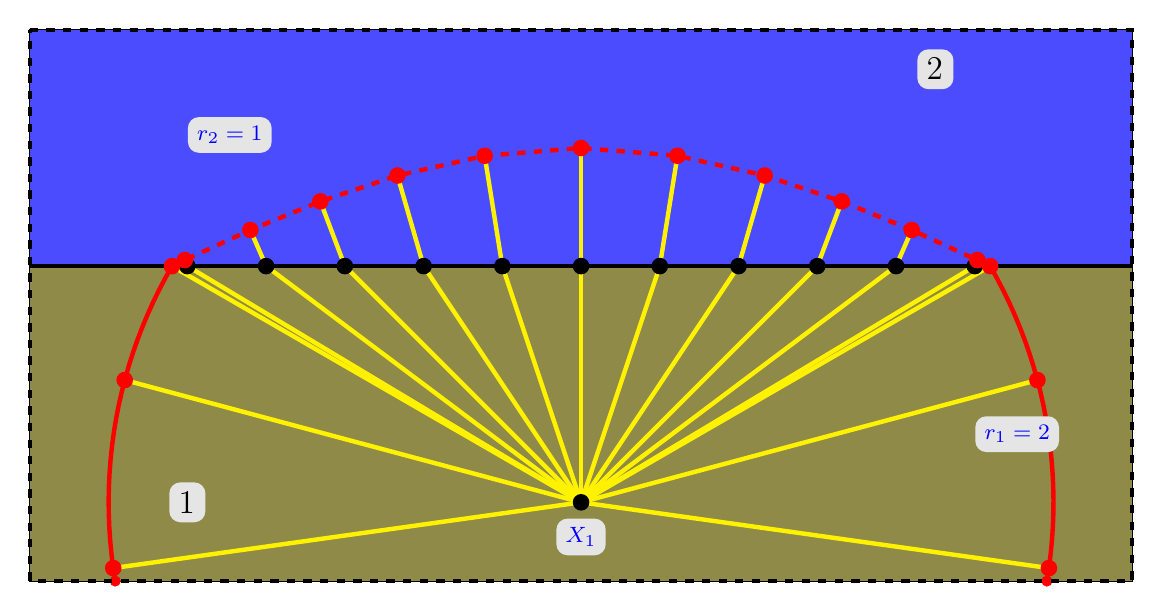
\begin{tikzpicture}


\coordinate (P1bdry) at (-7,3);
\coordinate (P2bdry) at (7,3);
\coordinate (P3bdry) at (-7,-4);
\coordinate (P4bdry) at (7,-4);
\coordinate (P1axis) at (-7,0);
\coordinate (P2axis) at (7,0);

\coordinate (X1) at (0,-3);
\coordinate (LL) at (-5.196,0);
\coordinate (Q0) at (-5,0);
\coordinate (Q1) at (-4,0);
\coordinate (Q2) at (-3,0);
\coordinate (Q3) at (-2,0);
\coordinate (Q4) at (-1,0);
\coordinate (Q5) atX1 (0,0);
\coordinate (Q6) at (1,0);
\coordinate (Q7) at (2,0);
\coordinate (Q8) at (3,0);
\coordinate (Q9) at (4,0);
\coordinate (Q00) at (5,0);
\coordinate (RR) at (5.196,0);
\coordinate (BLL) at (-5.916,-4);
\coordinate (BRR) at (5.916,-4);





%Upper Zone
\draw[fill = blue!70!]
(P1bdry) --  (P2bdry) -- (P2axis) -- (P1axis) -- cycle; 
%Lower Zone
\draw[fill = yellow!50!black]
(P1axis) --  (P2axis) -- (P4bdry) -- (P3bdry) -- cycle; 

%first part of traj
\draw[yellow,ultra thick] (X1) -- (LL);
\draw[yellow,ultra thick] (X1) -- (Q0);
\draw[yellow,ultra thick] (X1) -- (Q1);
\draw[yellow,ultra thick] (X1) -- (Q2);
\draw[yellow,ultra thick] (X1) -- (Q3);
\draw[yellow,ultra thick] (X1) -- (Q4);
\draw[yellow,ultra thick] (X1) -- (Q5);
\draw[yellow,ultra thick] (X1) -- (Q6);
\draw[yellow,ultra thick] (X1) -- (Q7);
\draw[yellow,ultra thick] (X1) -- (Q8);
\draw[yellow,ultra thick] (X1) -- (Q9);
\draw[yellow,ultra thick] (X1) -- (Q00);
\draw[yellow,ultra thick] (X1) -- (RR);

\draw[yellow,ultra thick] (X1) -- ++(15:6);
\draw[yellow,ultra thick] (X1) -- ++(-8:6);
\draw[yellow,ultra thick] (X1) -- ++(165:6);
\draw[yellow,ultra thick] (X1) -- ++(188:6);

\coordinate (X20) at (-5.03264, .0764);
\coordinate (X21) at (-4.2, .4583);
\coordinate (X22) at (-3.3107, .8219);
\coordinate (X23) at (-2.3321, 1.1503);
\coordinate (X24) at (-1.2243,1.401);
\coordinate (X25) at (0,1.5);
\coordinate (X26) at (1.2243,1.401);
\coordinate (X27) at (2.3321, 1.1503);
\coordinate (X28) at (3.3107, .8219);
\coordinate (X29) at (4.2, .4583);
\coordinate (X210) at (5.03264,.0764);


\draw[red,ultra thick,dashed] (LL)--(X20)--(X21)--(X22)--(X23)--(X24)--(X25)--(X26)--(X27)--(X28)--(X29)--(X210)--(RR);

%\shade[inner color=yellow, outer color=red] (LL)--(X20)--(X21)--
%(X22)--(X23)--(X24)--(X25)--(X26)--(X27)--(X28)--(X29)--(X210)--
%(RR)--;

%second part of traj
\draw[yellow,ultra thick] (Q0) -- (X20);
\draw[yellow,ultra thick] (Q1) -- (X21);
\draw[yellow,ultra thick] (Q2) -- (X22);
\draw[yellow,ultra thick] (Q3) -- (X23);
\draw[yellow,ultra thick] (Q4) -- (X24);
\draw[yellow,ultra thick] (Q5) -- (X25);
\draw[yellow,ultra thick] (Q6) -- (X26);
\draw[yellow,ultra thick] (Q7) -- (X27);
\draw[yellow,ultra thick] (Q8) -- (X28);
\draw[yellow,ultra thick] (Q9) -- (X29);
\draw[yellow,ultra thick] (Q00) -- (X210);


%Reachable set in M1
\draw [red,ultra thick,domain=150:189.6] plot ({6*cos(\x)}, {-3+6*sin(\x)});
\draw[ultra thick,red,domain=30:-9.6] plot ({6*cos(\x)},{-3+6*sin(\x)});

\fill[red] (-5.916,-4) circle (2pt);
\fill[red] (5.916,-4) circle (2pt);

%velocity balls

\node [blue, fill=gray!20, rounded corners,below right] at (5,-1.9){\footnotesize{$r_1=2$}} ;
\node [blue, fill=gray!20, rounded corners,below right] at (-5,1.9){\footnotesize{$r_2=1$}} ;

%labels of manifolds
\node [fill=gray!20, rounded corners] at (-5,-3){\LARGE{$\cM_1$}} ;
\node [fill=gray!20, rounded corners] at (4.5,2.5){\LARGE{$\cM_2$}} ;

%Boundaries
\draw[ultra thick,dashed] (P1bdry)  -- (P2bdry) -- (P4bdry) -- (P3bdry) -- cycle;
\draw[ultra thick] (P1axis) -- (P2axis);

\fill[black] (Q0) circle (3pt);
\fill[black] (X1) circle (3pt);
\fill[black] (Q1) circle (3pt);
\fill[black] (Q2) circle (3pt);
\fill[black] (Q3) circle (3pt);
\fill[black] (Q4) circle (3pt);
\fill[black] (Q5) circle (3pt);
\fill[black] (Q6) circle (3pt);
\fill[black] (Q7) circle (3pt);
\fill[black] (Q8) circle (3pt);
\fill[black] (Q9) circle (3pt);
\fill[black] (Q00) circle (3pt);

\fill[red] (LL) circle (3pt);
\fill[red] (X20) circle (3pt);
\fill[red] (X21) circle (3pt);
\fill[red] (X22) circle (3pt);
\fill[red] (X23) circle (3pt);
\fill[red] (X24) circle (3pt);
\fill[red] (X25) circle (3pt);
\fill[red] (X26) circle (3pt);
\fill[red] (X27) circle (3pt);
\fill[red] (X28) circle (3pt);
\fill[red] (X29) circle (3pt);
\fill[red] (X210) circle (3pt);
\fill[red] (RR) circle (3pt);

\fill[red] (X1)++(15:6) circle (3pt);
\fill[red] (X1)++(-8:6) circle (3pt);
\fill[red] (X1)++(165:6) circle (3pt);
\fill[red] (X1)++(188:6) circle (3pt);




%Points
\node [blue, fill=gray!20, rounded corners,below] at (0,-3.2) 
{\footnotesize{$X_1$}};



\end{tikzpicture}
\caption{Examples of \lq\lq optimal\rq\rq\ trajectories with $T=3$ in Case 1}
\label{fig: Case1}
\end{figure}

\[
\begin{array}{ll}
\begin{array}{l}
X_1=\begin{pmatrix} 0 \\ -3 \end{pmatrix},\,r_1=2,\,r_2=1 \\[12pt]
Q=\begin{pmatrix} x \\ 0\end{pmatrix} \\[12pt]
T_1= \gamma_{F_1}\bigl(Q-X_1\bigr)=\frac{\|Q-X_1\|}{2} \\[12pt]
\sin(\theta_1)=\frac{x}{\|Q-X_1\|} \\[12pt]
\sin\bigl(\theta_2\bigr)=\frac{r_2\,\sin(\theta_1)}{r_1}
=\frac{x}{2\,\|Q-X_1\|} \\[12pt]
\cos\bigl(\theta_2\bigr)=\frac{\sqrt{4\|Q-X_1\|^2-(x)^2}}{2\,\|Q-X_1\|} \\[12pt]
X_2=Q+(3-T_1)\begin{pmatrix} \sin(\theta_2) \\ \cos(\theta_2) \end{pmatrix} 
\end{array}
\qquad
&
\begin{array}{|c|c|c|c|c|c|}
\hline\hline
\vphantom{\biggl\{\biggl\}}\hphantom{\quad}x\hphantom{\quad} & \hphantom{\quad}T_1\hphantom{\quad} & \hphantom{\;}\sin\bigl(\theta_1\bigr)\hphantom{\;} & \hphantom{\;}\sin\bigl(\theta_2\bigr)\hphantom{\;} &\hphantom{\;}\cos(\theta_2)\hphantom{\;} & X_2 \\\hline\hline
-5 &\frac{\sqrt{34}}{2} & \frac{-5}{\sqrt{34}
} & \frac{-5}{2\sqrt{34}} & \frac{1}{2}\sqrt{\frac{111}{34}} & \begin{pmatrix} -5.03264 \\ 
.0764\end{pmatrix}   \\[5pt]\hline
-4 & \frac{5}{2}& \frac{-4}{5} & \frac{-2}{5} & 
\frac{\sqrt{21}}{5} & \begin{pmatrix}  -4.2\\ .4583 \end{pmatrix}  \\\hline
-3 & \frac{\sqrt{18}}{2} & \frac{-3}{\sqrt{18}} & \frac{-3}{2\sqrt{18}} & \sqrt{\frac{63}{72}} & \begin{pmatrix}  -3.3107\\ .8219 \end{pmatrix} \\\hline
-2 & \frac{\sqrt{13}}{2} & \frac{-2}{\sqrt{13}} & \frac{-1}{\sqrt{13}} & \sqrt{\frac{48}{52}}& \begin{pmatrix}  -2.3321 \\ 1.1503 \end{pmatrix} \\\hline
-1 &
\frac{\sqrt{10}}{2}& \frac{-1}{\sqrt{10}} & \frac{-1}{2\sqrt{10}}&
\sqrt{\frac{39}{40}} & \begin{pmatrix}  -1.2243 \\ 1.401 \end{pmatrix}
 \\\hline
0  & \frac{3}{2} & 0 & 0 & 1 & \begin{pmatrix} 0 \\ 3\slash 2\end{pmatrix} \\\hline\hline
\end{array}
\end{array}
\]

\noindent
The optimal velocity in the first part of the trajectory is
$v_1=\frac{2\bigl(Q-X_1\bigr)}{\|Q-X_1\|} $,
and in the second part is $v_2=\frac{X_2-Q}{\bigl(Q-X_1\bigr)}$.



\bigskip


\noindent
{\bf Case 2:}  Now let us specify $F_1=\ball$, $F_2=2\ball$, and $X_1=\begin{pmatrix}0 \\ -3\end{pmatrix}$; similar considerations apply for any $0<r_1<r_2$ and $X_1\in\cM_1$.  When $0\leq T\leq 3$ the reachable set is just $X+T\ball$.  When $T>3$, it becomes more interesting because there are now three separate types of an optical arc.  

\noindent{\bf Subcase 2a:}  A trajectory never leaves $\cM_1$.  In particular, every point in $\cM_1\bigcap \bigl\{X_1+ T\ball\bigr\}$ belongs to $R^{(T)}(X_1)$, although as we'll see, not all of the boundary points belong to the boundary of $R^{(T)}(X_1)$.  

\noindent{\bf Subcase 2b:}  A trajectory leaves $\cM_1$ and spends the remaining time in $\cM_2$; this is the analyzed in a manner similar to Case 1, and produces those points in $\cM_2\bigcap R^{(T)}(X_1)$.  Examples are shown in Figure~\ref{fig: Cases 2a and 2b} with $T=6$. 

\begin{figure}[h]
\centering
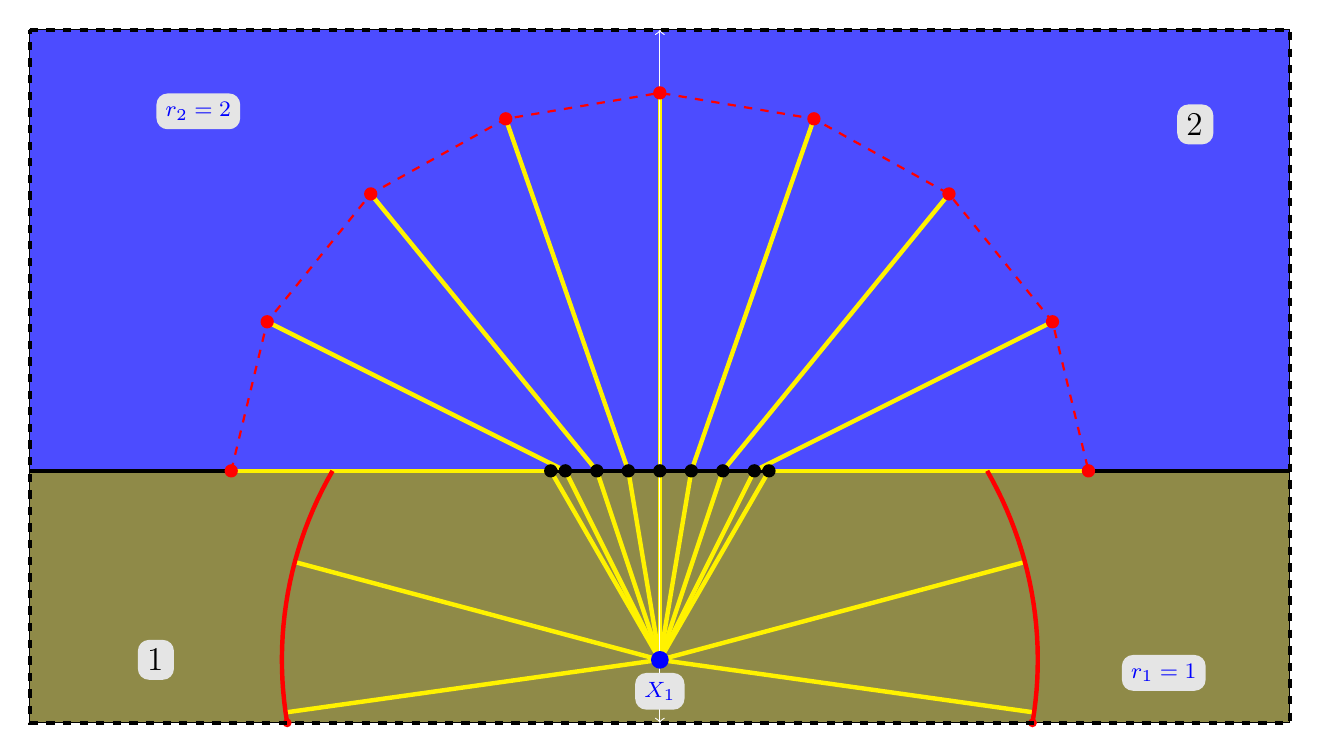
\begin{tikzpicture}[scale=.8]


\coordinate (P1bdry) at (-10,7);
\coordinate (P2bdry) at (10,7);
\coordinate (P3bdry) at (-10,-4);
\coordinate (P4bdry) at (10,-4);
\coordinate (P1axis) at (-10,0);
\coordinate (P2axis) at (10,0);


\coordinate (X1) at (0,-3);
\coordinate (Q0) at (0,0);
\coordinate (Q1) at (.5,0);
\coordinate (Q2) at (1,0);
\coordinate (Q3) at (1.5,0);
\coordinate (Q4) at (1.732,0);
\coordinate (Q-1) at (-.5,0);
\coordinate (Q-2) at (-1,0);
\coordinate (Q-3) at (-1.5,0);
\coordinate (Q-4) at (-1.732,0);





%Upper Zone
\draw[fill = blue!70!]
(P1bdry) --  (P2bdry) -- (P2axis) -- (P1axis) -- cycle; 
%Lower Zone
\draw[fill = yellow!50!black]
(P1axis) --  (P2axis) -- (P4bdry) -- (P3bdry) -- cycle; 
\draw[ultra thick] (P1axis) -- (P2axis);

%first part of traj
\draw[yellow,ultra thick] (X1) -- (Q0);
\draw[yellow,ultra thick] (X1) -- (Q1);
\draw[yellow,ultra thick] (X1) -- (Q2);
\draw[yellow,ultra thick] (X1) -- (Q3);
\draw[yellow,ultra thick] (X1) -- (Q4);
\draw[yellow,ultra thick] (X1) -- (Q-1);
\draw[yellow,ultra thick] (X1) -- (Q-2);
\draw[yellow,ultra thick] (X1) -- (Q-3);
\draw[yellow,ultra thick] (X1) -- (Q-4);

\draw[yellow,ultra thick] (X1) -- ++(15:6);
\draw[yellow,ultra thick] (X1) -- ++(-8:6);
\draw[yellow,ultra thick] (X1) -- ++(165:6);
\draw[yellow,ultra thick] (X1) -- ++(188:6);

%Subcase 2b boundary points
\coordinate (X2 0) at (0,6);
\coordinate (X2 1) at (2.4456,5.5882);
\coordinate (X2 2) at (4.5894,4.3961);
\coordinate (X2 3) at (6.2331, 2.3666);
\coordinate (X2 4) at (6.8038, 0);
\coordinate (X2-1) at (-2.4456,5.5882);
\coordinate (X2-2) at (-4.5894,4.3961);
\coordinate (X2-3) at (-6.2331, 2.3666);
\coordinate (X2-4) at (-6.8038, 0);

\draw[red, thick, dashed] (X2-4)--(X2-3)--(X2-2)--(X2-1)--(X2 0)--(X2 1)--(X2 2)--(X2 3)--(X2 4); 



%\draw[red,ultra thick,dashed] (LL)--(X20)--(X21)--(X22)--(X23)--(X24)--(X25)--(X26)--(X27)--(X28)--(X29)--(X200)--(RR);
%
%\shade[inner color=yellow, outer color=red] (LL)--(X20)--(X21)--
%(X22)--(X23)--(X24)--(X25)--(X26)--(X27)--(X28)--(X29)--(X200)--
%(RR)--;

%second part of traj

\draw[yellow,ultra thick] (Q0) -- (X2 0);
\draw[yellow,ultra thick] (Q1) -- (X2 1);
\draw[yellow,ultra thick] (Q2) -- (X2 2);
\draw[yellow,ultra thick] (Q3) -- (X2 3);
\draw[yellow,ultra thick] (Q4) -- (X2 4);
\draw[yellow,ultra thick] (Q0) -- (X2 0);
\draw[yellow,ultra thick] (Q-1) -- (X2-1);
\draw[yellow,ultra thick] (Q-2) -- (X2-2);
\draw[yellow,ultra thick] (Q-3) -- (X2-3);
\draw[yellow,ultra thick] (Q-4) -- (X2-4);


%Reachable set in M1
\draw [red,ultra thick,domain=150:189.6] plot ({6*cos(\x)}, {-3+6*sin(\x)});
\draw[ultra thick,red,domain=30:-9.6] plot ({6*cos(\x)},{-3+6*sin(\x)});

\fill[red] (-5.916,-4) circle (2pt);
\fill[red] (5.916,-4) circle (2pt);

%velocity balls

\node [blue, fill=gray!20, rounded corners,above] at (8,-3.5){\footnotesize{$r_1=1$}} ;
\node [blue, fill=gray!20, rounded corners,below right] at (-8,6){\footnotesize{$r_2=2$}} ;

%labels of manifolds
\node [fill=gray!20, rounded corners] at (-8,-3){\LARGE{$\cM_1$}} ;
\node [fill=gray!20, rounded corners] at (8.5,5.5){\LARGE{$\cM_2$}} ;

%Boundaries
\draw[ultra thick,dashed] (P1bdry)  -- (P2bdry) -- (P4bdry) -- (P3bdry) -- cycle;
%\draw[ultra thick] (P1axis) -- (P2axis);
\draw[<->,white, thin] (0,-4) -- (0,7);

\fill[black] (Q0) circle (3pt);
\fill[black] (Q1) circle (3pt);
\fill[black] (Q2) circle (3pt);
\fill[black] (Q3) circle (3pt);
\fill[black] (Q4) circle (3pt);
\fill[black] (Q-1) circle (3pt);
\fill[black] (Q-2) circle (3pt);
\fill[black] (Q-3) circle (3pt);
\fill[black] (Q-4) circle (3pt);



\fill[red] (X2 0) circle (3pt);
\fill[red] (X2 1) circle (3pt);
\fill[red] (X2 2) circle (3pt);
\fill[red] (X2 3) circle (3pt);
\fill[red] (X2 4) circle (3pt);
\fill[red] (X2-1) circle (3pt);
\fill[red] (X2-2) circle (3pt);
\fill[red] (X2-3) circle (3pt);
\fill[red] (X2-4) circle (3pt);

\fill[blue] (X1) circle (4pt);


%Points
\node [blue, fill=gray!20, rounded corners,below] at (0,-3.2) 
{\footnotesize{$X_1$}};



\end{tikzpicture}
\caption{Examples of optimal trajectories of Subcases 2a and 2b}
\label{fig: Cases 2a and 2b}
\end{figure}

\noindent{\bf Subcase 2c:}  An optimal trajectory may hit $\Sigma$ at some time $T_1<T$, and stay on $\Sigma$ until time $T_2$ and then re-enter $\cM_1$. 

\begin{figure}[h]
\centering
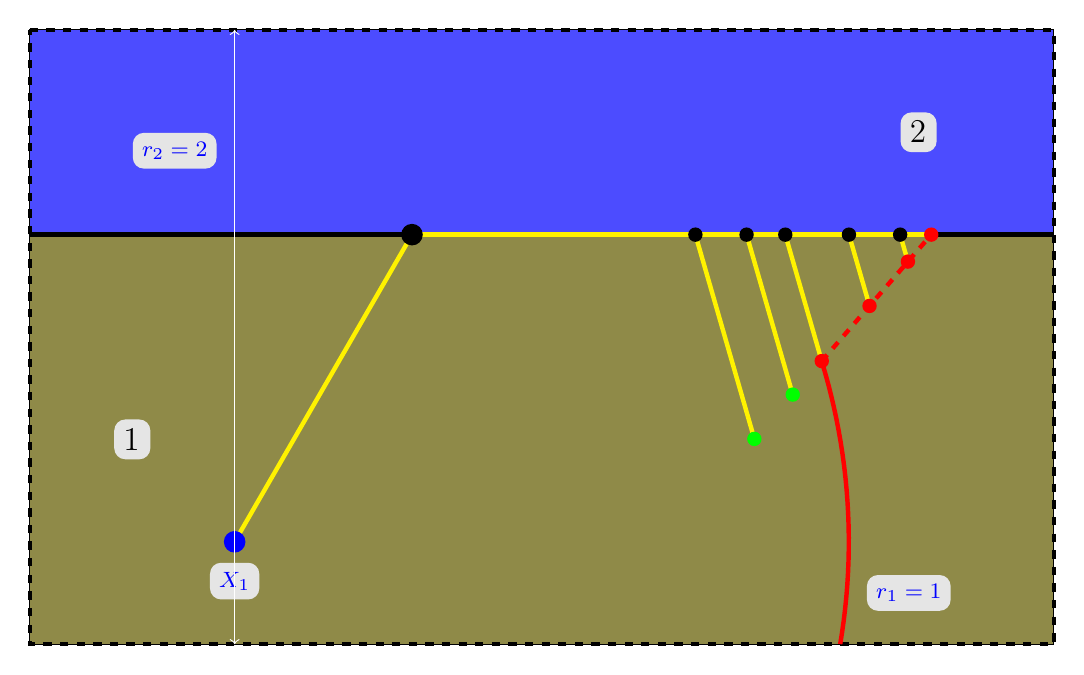
\begin{tikzpicture}[scale=1.3]


\coordinate (P1bdry) at (-2,2);
\coordinate (P2bdry) at (8,2);
\coordinate (P3bdry) at (-2,-4);
\coordinate (P4bdry) at (8,-4);
\coordinate (P1axis) at (-2,0);
\coordinate (P2axis) at (8,0);

\coordinate (X1) at (0,-3);
\coordinate (Q1) at (1.732,0);
\coordinate (Q2 1) at (4,0);
\coordinate (Q2 2) at (4.5,0);
\coordinate (Q2 3) at (5,0);
\coordinate (Q2 4) at (5.3781,0);
\coordinate (Q2 5) at (6,0);
\coordinate (Q2 6) at (6.5,0);
\coordinate (Q2 7) at (6.803848,0);



%Upper Zone
\draw[fill = blue!70!]
(P1bdry) --  (P2bdry) -- (P2axis) -- (P1axis) -- cycle; 
%Lower Zone
\draw[fill = yellow!50!black]
(P1axis) --  (P2axis) -- (P4bdry) -- (P3bdry) -- cycle; 

%Boundaries
\draw[ultra thick,dashed] (P1bdry)  -- (P2bdry) -- (P4bdry) -- (P3bdry) -- cycle;
\draw[ultra thick] (P1axis) -- (P2axis);

%first part of traj
\draw[yellow,ultra thick] (X1) -- (Q1);
\draw[yellow,ultra thick] (Q1) -- (Q2 7);

%Subcase 2b boundary points
\coordinate (X2 1) at (5.2141,-.7009);
\coordinate (X2 2) at (5.076,-1.995);
\coordinate (X2 3) at (5.451,-1.5622);
\coordinate (X2 4) at (5.7345,-1.2347);
\coordinate (X2 5) at (6.201,-.69615);
\coordinate (X2 6) at (6.576,-.26314);


%second part of traj

\draw[yellow,ultra thick] (Q2 2) -- (X2 2);
\draw[yellow,ultra thick] (Q2 3) -- (X2 3);
\draw[yellow,ultra thick] (Q2 4) -- (X2 4);
\draw[yellow,ultra thick] (Q2 5) -- (X2 5);
\draw[yellow,ultra thick] (Q2 6) -- (X2 6);



\fill[black] (Q1) circle (3pt);
\draw[ultra thick,red,domain=17.1106:-9.6] plot ({6*cos(\x)},{-3+6*sin(\x)});


%velocity balls

\node [blue, fill=gray!20, rounded corners,left] at (7,-3.5){\footnotesize{$r_1=1$}} ;
\node [blue, fill=gray!20, rounded corners,below right] at (-1,1){\footnotesize{$r_2=2$}} ;

%labels of manifolds
\node [fill=gray!20, rounded corners] at (-1,-2){\LARGE{$\cM_1$}} ;
\node [fill=gray!20, rounded corners,right] at (6.5,1){\LARGE{$\cM_2$}} ;

\draw[red,dashed,ultra 
thick] (X2 4) -- (X2 5) -- (X2 6) -- (Q2 7);



\fill[black] (Q1) circle (2pt);
%\fill[black] (Q2 1) circle (2pt);
\fill[black] (Q2 2) circle (2pt);
\fill[black] (Q2 3) circle (2pt);
\fill[black] (Q2 4) circle (2pt);
\fill[black] (Q2 5) circle (2pt);
\fill[black] (Q2 6) circle (2pt);
\fill[red] (Q2 7) circle (2pt);

%\fill[green] (X2 1) circle (2pt);
\fill[green] (X2 2) circle (2pt);
\fill[green] (X2 3) circle (2pt);
\fill[red] (X2 4) circle (2pt);
\fill[red] (X2 5) circle (2pt);
\fill[red] (X2 6) circle (2pt);

\fill[blue] (X1) circle (3pt);

%Points
\node [blue, fill=gray!20, rounded corners,below] at (0,-3.2) 
{\footnotesize{$X_1$}};
\draw[white,<->,thin] (0,-4) -- (0,2);


\end{tikzpicture}
\caption{\parbox{5in}{Examples of trajectories in Subcase 2c.  Points at the end of optimal arcs are red, and those in the interior of $R^{(6)}(X_1)$ are green.}}\label{fig: Case2c}
\end{figure}



\[
\begin{array}{ll}
\begin{array}{l}
X_1=\begin{pmatrix} 0 \\ -3 \end{pmatrix},\,r_1=1,\,r_2=2 \\[12pt]
Q_1=\begin{pmatrix} \sqrt{3} \\ 0\end{pmatrix};\quad 
Q_2=\begin{pmatrix} x \\ 0\end{pmatrix}\\[15pt]
T_1=\sqrt{12}\;;\quad T_2= T_1+\frac{1}{2}\bigl(x-\sqrt{3}\bigr)
 \\[12pt]
X_2=\begin{pmatrix} x_2 \\ y_2\end{pmatrix} = Q_2+
\frac{1}{2}(6-T_2)\begin{pmatrix} 1 \\ -\sqrt{3} \end{pmatrix} 
\end{array}
\qquad
&
\begin{array}{||c|c|c|c||}
\hline\hline
\vphantom{\biggl\{\biggr\}}x & T_2 & X_2 & \bigl\|X_2-X_1\bigr\|\\\hline\hline
%4 & 4.598 & \begin{pmatrix} 5.2141 \\ -.7009\end{pmatrix} & 5.6985\\
%\hline
4.5 & 4.848 & \begin{pmatrix} 5.076 \\ -1.995\end{pmatrix}& 5.1745 \\\hline
5  & 5.098 & \begin{pmatrix} 5.451 \\ -1.5622\end{pmatrix} & 5.6374\\\hline
5.3781 & 5.2871 & \begin{pmatrix} 5.7345 \\ -1.2347\end{pmatrix} & 6\\\hline
6  & 5.598 & \begin{pmatrix} 6.201 \\ -.69615\end{pmatrix} & 6.6151\\\hline
6.5  & 5.848 & \begin{pmatrix} 6.576 \\ -.26314\end{pmatrix} & 7.123\\\hline
6.8038 & 6 & \begin{pmatrix} 6.8038 \\ 0\end{pmatrix} & 7.4359
\\
\hline\hline
\end{array}
\end{array}
\]
The full reachable set is the union of all the trajectories coming from one of the subcases.  The boundary of the reachable set would typically consist of all endpoints of one of the optimal trajectories, but his is not necessarily the case as seen by the green points in Figure~\ref{fig: Case2c}.

\section{Moving faster on $\Sigma$}
We looked in Subcase 2c above at a trajectory moving on the interface $\Sigma$, but we assumed that that speed was the same as the subspace.  We next consider the possibility that $\Sigma$ is like a road or a boardwalk in which faster movement is possible. 
Suppose the interface $\Sigma$ also has a velocity set $G$.  The velocity set $G$ restricts the motion on $\Sigma$, and $G$ is assumed to be closed, convex, and satisfying $\langle \vec n,G\rangle:=\bigl\{\langle \vec n,v\rangle:\;v\in G\bigr\}=\{0\}$.  The latter requirement is needed so that for any trajectory that begins on $\Sigma$ moving with a velocity in $G$ stays on $\Sigma$.  The assumption (H1) now needs a slight modification since obviously the interior of $G$ in $\R^n$ is empty.  The modification of (H1) is to require there exists $\delta>0$ so that $\Sigma\cap\delta\ball\subseteq G$, or that $0$ belongs to the {\it relative interior} of $G$.  We will always assume
\begin{equation*}\tag{H2}
\bigl[F_1\bigcup F_2\bigr]\bigcap \Sigma\subseteq G,
\end{equation*}
which in effect says that any movement just off of $\Sigma$ can be done at least as fast as being on $\Sigma$.


{\blue
\begin{exer}\label{Ex: probs}
\begin{itemize}
\item[(a)]  Consider the case where $X_1\in\cM_1$ and $X_2\in\cM_2$.
Show that (P1) is equivalent to the problem
\begin{equation*}\tag*{\begin{color}{black}($\cP3$)\end{color}}
\min\;J\bigl(Q_1,\,Q_2\bigr)\quad\text{over }Q_1,\,Q_2\in\R^n,
\end{equation*}
where
\[
J\bigl(Q_1,\,Q_2\bigr):=\biggl\{\gamma_{F_1}(Q_1-X_1)+\gamma_{G}(Q_2-Q_1)+\gamma_{F_2}(X_2-Q_2) +\cI_{\Sigma}(Q_1)+\cI_{\Sigma}(Q_2)\biggr\}
\]
\item[(b)]  In the case where $X_1\in\cM_1$ and $X_2\in\Sigma$, show that $(\cP1)$ is equivalent to $(\cP2)$.
\item[(c)]  In the case where both $X_1$ and $X_2$ belong to $\cM_1$, show there are at most two types of optimal solutions, and
\[
\min(\cP)=\min\bigl\{\min(\cP3),\gamma_{G}(X_2-X_1)\bigr\}.
\] 
\end{itemize}
\end{exer}}

We make some simple observations in the case where each velocity set is a ball $r\ball$ where $r>0$.  To fix notation, suppose $F_i=r_i\ball$, $i=1,\,2$, and on the interface $\Sigma$, $G=\Sigma\cap r_3\ball$.  Assumption (H2) in this case is equivalent to assuming $r_3\geq\max\{r_1,\,r_2\}$.

{\blue
\begin{exer}
\begin{itemize}
\item[(a)]  If $r_3\leq\min\{r_1,\,r_2\}$, show that for
 any $X_1\in\cM_1$ and $X_2\in\cM_2$, an optimal solution to ($\cP3$) has $Q_1=Q_2$.  That is, any optimal trajectory spends no time on the interface $\Sigma$.
\item[(b)]  Give an example in $\R^2$ (i.e. produce $X_1,\,X_2\in\R^2$ and $r_1,\,r_2,\,r_3>0$) where the solution to ($\cP3$) has $Q_1\not= Q_2$.
\item[(c)]  Suppose  $r_1,\,r_2,\,r_3>0$ with $r_3>\max\{r_1,r_2\}$, characterize those points $X_1\in\cM_1$ and $X_2\in\cM_2$ for which $Q_1=Q_2$. 
\end{itemize}
\end{exer}
}

The necessary (and sufficient) conditions for $Q_1$ and $Q_2$ to solve ($\cP3$) are the existence of $\zeta_i\in\R^n$, $i=1,\,2,\,3,\,4$, so that
\[
\begin{array}{rclrcl}
\zeta_1 & \; \in \; & \partial\gamma_{F_1}(Q_1-X_1) \qquad\qquad\qquad 
&\zeta_3 & \in & \partial\gamma_{G}(Q_2-Q_1)   \\
-\zeta_2 & \in &\partial\gamma_{G}(Q_2-Q_1) 
&-\zeta_4 & \in & \partial\gamma_{F_2}(X_2-Q_2)  \\ 
\zeta_1-\zeta_2 & \in & N_{\Sigma}(Q_1) 
&\zeta_3-\zeta_4 & \in & N_{\Sigma}(Q_2)  
\end{array}
\]
which imply
\begin{equation}\label{eq: 2polar = 1}
\gamma_{F_1^{\circ}}(\zeta_1)=
\gamma_{G^{\circ}}(-\zeta_2)=
\gamma_{G^{\circ}}(\zeta_3)= 
\gamma_{F_2^{\circ}}(-\zeta_4)=1.
\end{equation}
The optimal velocities are
\[
v_1:=\frac{Q_1-X_1}{\gamma_{F_1}(Q_1-X_1)}\in F_1 \qquad 
u=\frac{Q_2-Q_1}{\gamma_{G}(Q_2-Q_1)}\in G \qquad
v_2:=\frac{X_2-Q_2}{\gamma_{F_2}(X_2-Q_2)}\in F_2
\]
and the Max Principle says
\begin{align}
v\mapsto \langle\zeta_1,v\rangle\quad &\text{is maximized over }v\in F_1\text{ at } v=v_1 \label{eq: 2MP1}\\
v\mapsto \langle-\zeta_2,v\rangle\quad &\text{is maximized over }v\in G\text{ at } v=u. \label{eq: 2MP2} \\
v\mapsto \langle\zeta_3,v\rangle\quad &\text{is maximized over }v\in G\text{ at } v=u \label{eq: 2MP3}  \\
v\mapsto \langle-\zeta_4,v\rangle\quad &\text{is maximized over }v\in F_2\text{ at } v=v_2 \label{eq: 2MP4}
\end{align}


\begin{Exam}\label{Example 2}
{\rm
Again consider the case with $n=2$, $\cM_1$ the lower half space with velocity set $F_1=r_1\ball$, $\cM_2$ the upper half space with velocity set $F_2=r_2\ball$, and $\Sigma$ the $x$-axis with velocity set $G=\Sigma\bigcap r_3\ball$.  Consider ($\cP1$) with $X_1\in\cM_1$ and $X_2\in\cM_2$, and sufficiently far apart so that $Q_1\not=Q_2$ --- see Figure~\ref{fig: Snell2}.
}
\end{Exam}

\begin{figure}[h]\label{fig: Snell2}
\centering
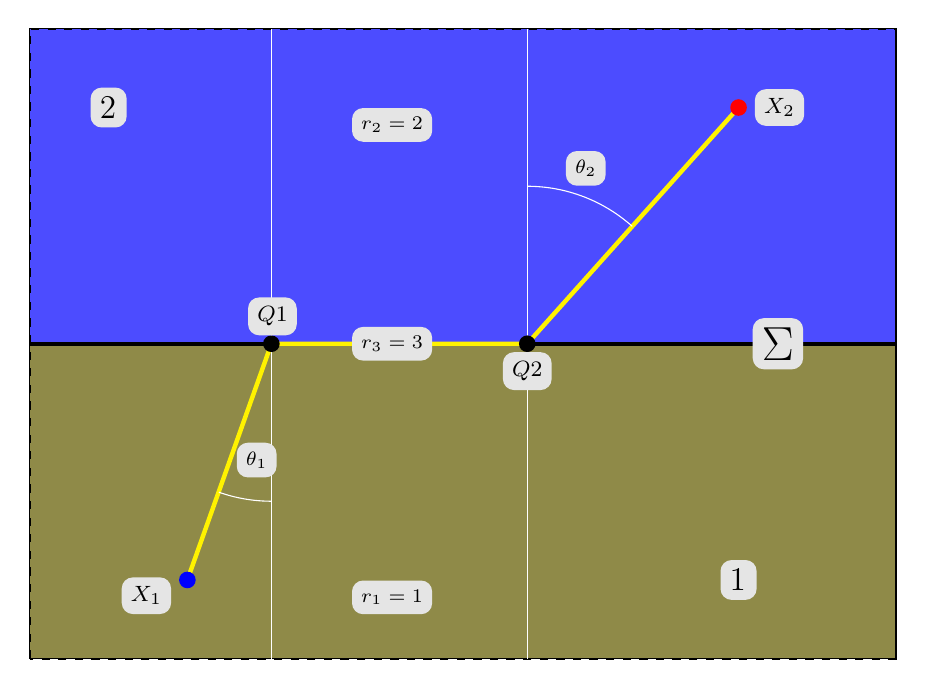
\begin{tikzpicture}


\coordinate (P1bdry) at (-2,-4);
\coordinate (P2bdry) at (-2,4);
\coordinate (P3bdry) at (9,4);
\coordinate (P4bdry) at (9,-4);

\coordinate (P1axis) at (-2,0);
\coordinate (P2axis) at (9,0);

\coordinate (X1) at (0,-3);
\coordinate (X2) at (7,3);

\coordinate (Q1) at (1.067,0);
\coordinate (Q2) at (4.3167,0);



%Upper Zone
\draw[fill = blue!70!]
(P2bdry) --  (P3bdry) -- (P2axis) -- (P1axis) -- cycle; 
%Lower Zone
\draw[fill = yellow!50!black]
(P1axis) --  (P2axis) -- (P4bdry) -- (P1bdry) -- cycle; 
\draw[ultra thick,black] (P1axis) -- (P2axis);


%Opt trajectory
\draw[yellow,ultra thick] (X1) -- (Q1) -- (Q2) -- (X2);

%labels of manifolds
\node [fill=gray!20, rounded corners] at (7,-3){\LARGE{$\cM_1$}} ;
\node [fill=gray!20, rounded corners] at (-1,3){\LARGE{$\cM_2$}} ;
\node [fill=gray!20, rounded corners] at (7.5,0){\LARGE{$\Sigma$}} ;


%Boundaries
\draw[thick,dashed] (P1bdry)  -- (P2bdry) -- (P3bdry) -- (P4bdry) -- cycle;


%angles
\draw[white, thin] (1.067,-4) -- (1.067,4);
\draw[white, thin] (4.3167,-4) -- (4.3167,4);
\draw[white, thin] (1.067,-2) arc (-90:-109.4712:2);
\node [black, fill=gray!20, rounded corners,above right] at (4.8,2)
{\scriptsize{$\theta_2$}};
\draw[white, thin] (4.3167,2) arc (90:48.1897:2);
\node [black, fill=gray!20, rounded corners,below] at (.88,-1.25)
{\scriptsize $\theta_1$};

%points
\fill[blue] (X1) circle (3pt);
\fill[black] (Q1) circle (3pt);
\fill[black] (Q2) circle (3pt);
\fill[red] (X2) circle (3pt);
\node [black, fill=gray!20, rounded corners,left] at (-.2,-3.2) 
{\footnotesize{$X_1$}};
\node [black, fill=gray!20, rounded corners,right] at (7.2,3) 
{\footnotesize{$X_2$}};
\node [black, fill=gray!20, rounded corners,above] at (1.08,.1){\footnotesize{$Q1$}} ;
\node [black, fill=gray!20, rounded corners,below] at (4.3167,-.1){\footnotesize{$Q2$}} ;

\node [black, fill=gray!20, rounded corners,below] at (2.6,3) 
{\scriptsize{$r_2=2$}};
\node [black, fill=gray!20, rounded corners] at (2.6,0) 
{\scriptsize{$r_3=3$}};
\node [black, fill=gray!20, rounded corners,below] at (2.6,-3) 
{\scriptsize{$r_1=1$}};


\end{tikzpicture}
\caption{Case 1 where $Q_1\not= Q_2$}
\end{figure}
Snell's Law now operates at both switching points $Q_1$ and $Q_2$, and the incidental angles
 satisfy
\begin{equation}\label{eq: 2pt Snell}
\sin(\theta_1)=\frac{r_1}{r_3}\quad\text{and}\quad
\sin(\theta_2)=\frac{r_2}{r_3}.
\end{equation}
We now address the issue when $X_1:=\begin{pmatrix} x_1 \\ y_1\end{pmatrix}$ and  $X_2:=\begin{pmatrix} x_2 \\ y_2\end{pmatrix}$  are such that the corresponding $Q_i$'s are different.  For definiteness, suppose the situation is similar to what is shown in Figure~\ref{fig: Snell2} where $y_1<0<y_2$ and $x_1\leq x_2$.  We write $Q_i:=\begin{pmatrix} q_i \\ 0\end{pmatrix}$, and we want to characterize when $q_1\leq q_2$.  This happens if and only if \eqref{eq: 2pt Snell} holds, and the values $q_i$ can be directly calculated from this information.  The conclusion is that $Q_1\not=Q_2$ if and only if
\[
x_1+(-y_1)\tan\left(\inv{\sin}\left(\frac{r_1}{r_3}\right)\right)
< x_2+(y_2)\tan\left(\inv{\sin}\left(\frac{r_2}{r_3}\right)\right).
\]

{\blue
\begin{exer}
Consider the examples in Exercise~\ref{exer: examples} where we now add the velocity set $G:=\left\{\begin{pmatrix} u \\ 0 \end{pmatrix}:\;|u|\leq 3\right\}$ on the interface $\Sigma$.  Solve (P3) for each of (a)-(d).
\end{exer}
}





%\section{Dynamic Programming}


\end{document}







\begin{defn}
A vector $\zeta\in X$ is called an {\em $F$-normal} to a point
$\bar s\in S$ provided there exists a $\delta>0$ satisfying
\[
\Biggl\{\bar s + \delta\frac{1}{\gamma_F(-\zeta)}\zeta
+\delta'F\biggr\} \cap S =\emptyset
     \quad \forall \;\delta'\in(0,\delta),

\]
in which case we say that $\zeta$ is {\em realized} by $\delta$.
The set of all $F$-normals at the point $\bar s\in S$ is denoted
by $ N_{S}^{F}(\bar s)$.  Furthermore, we write $\Pi^{F}_{S}(\bar
x)$ for the set of all $F$-projections onto $S$:
\[
\Pi^{F}_{S}(\bar x):=S\cap \{\bar x + T_S(\bar x)F\}.
\]
\end{defn}


\begin{exer}
Show that
\begin{enumerate}
\item[(a)] $T_S^F(x)=\inf_{s\in S}\gamma_F(s-x)=\gamma_F(z-x)$ for all $z\in
\psf (x)$;
\item[(b)] $T_S^F(x)-T_S^F(y)\le \gamma_F(y-x)$;
\item[(c)] for all $x,y\not\in S$,
\[
\left| T_S^F(x)-T_S^F(y) \right| \le \max\{ \rf (y-x),\rf
(x-y)\}\le \displayfrac{\| y-x\|}{r};
\]
\item[(d)] Suppose $\bar x\not\in S$, and assume that
$\psf(x)$ is a singleton for all $x$ in a neighborhood of $\bar
x$; then $x\to\psf(x)$ is continuous in the same neighborhood. Is
it also locally Lipschitz ??
\end{enumerate}
\end{exer}

\begin{rem}

\begin{enumerate}
\item[1.]  If $F$ equals the unit ball $\ball$ in $X$,
then the set of $F$-normals equals the proximal normal cone.
\item[2.]  Even if $S$ has smooth boundary, the set
$ N_{S}^{F}(\bar s)$ may contain more than a half line.
\end{enumerate}
\end{rem}


\begin{prop}
If $X$ is finite dimensional and $S$ is convex, then
$N^F_S(s)\not=\emptyset$ for all $s\in\bd S$, and every $\zeta\in
N^F_S(s)$ is realized by every $\delta>0$.
\end{prop}
{\em Proof:}  Suppose $\bar s\in\bd S$, where $S$ is convex.
Without loss of generality we may assume $\bar s=0$.  Let $\xi$
belong to the convex normal cone of $S$ at $\bar s=0$.  Then
$\langle \xi,s\rangle\leq 0$ for all $s\in S$.  Choose $-\zeta\in
F$ so that
\[
\langle-\zeta,\xi\rangle = \min_{v\in F}\langle v,\xi\rangle,
\]
the above quantity being necessarily negative since $0\in \iint
F$. We claim that $\zeta\in N^F_S(0)$ and is realized by any
$\delta>0$. Indeed, note that $-\zeta\in \bd F$, and so
$\gamma_F(-\zeta)=1$. Let $0<\delta'<\delta$, and suppose there
exists $s=\delta\zeta+\delta'v \in S\cap\biggl[\delta\zeta +
\delta'F\biggr]$.  Then $\langle\xi,s\rangle\leq 0$ since $\xi$ is
in the convex normal cone at $0$ and $s\in S$.  On the other hand,
\[
\langle s,\xi\rangle = \delta\langle\zeta,\xi\rangle
+\delta'\langle v,\xi\rangle>0
\]
since $\langle\zeta,\xi\rangle=\max_{v\in F}\langle v,\xi\rangle$
and $0\leq\delta'<\delta$.  This contradiction leads to the
conclusion that $\zeta\in N_{S}^{F}(0)$.
 \eop




%%%%%%%%%%%%%%%%%%%%%%%%%%%%%%%%%%%%%%%%%%%%%%%%%%%%%%%%



%%%%%%%%%%%%%%%%%%%%%%%%%%%%%%%%%%%%%%%%%%%%%%%%%%%%%%%%

The study of the differentiability properties of $T_S(\cdot)$
requires the following concept.

\begin{defn}
Suppose $\bar x\notin S$, and $\bar s\in \Pi^{F}_{S}(\bar x)$.
The $S\slash F$ separating normal cone $\sep (S\slash F, \bar
s,\bar x)$ for $(\bar s,\bar x)$ is defined by
\[
\sep(S\slash F, \bar s,\bar x):=N^{C}_{S}(\bar s)\cap
\biggl\{-N_{F}\left(\frac{\bar s-\bar x}{\gamma_{F}(\bar s-\bar
x)}\right)\biggr\},
\]
where $N^{C}_{S}(\bar s)$ is the Clarke normal cone at $\bar s$
and $N_{F}(v)$ denotes the convex normal cone at $v\in F$.
\end{defn}

\begin{rem}
Suppose $\bar s\in\Pi^F_S(\bar x)$, and $\bar x-\bar s$ is
realized by $\delta>0$.  If $S$ is (Clarke) regular, then $\vec
n\in\sep(S\slash F,\bar s,\bar x)$ if and only if the following
two properties hold:
\begin{itemize}
\item[(i)]
\[
\limsup_{\begin{array}{c}
\begin{scriptsize} s\to \bar s \end{scriptsize}\\
\begin{scriptsize} s\in S \end{scriptsize}
\end{array}}
\left\langle \vec
n,\frac{s-\bar s}{\|s-\bar s \|}\right\rangle\leq 0,
\]
\item[(ii)]
\[
\bar s + \delta\left[\frac{\bar x - \bar s}{\gamma_F(\bar s -\bar
x)}+F\right] \subseteq \biggl\{x:\langle \vec n,x-\bar
s\rangle\geq 0\biggr\}.
\]
\end{itemize}
Indeed, (i) says that $\vec n\in N^C_S(\bar s)$ and (ii) is
equivalent to $-\vec n\in N_F\left(\frac{\bar s-\bar
x}{\gamma_F(\bar s-\bar x)}\right)$.
\end{rem}

%%%%%%%%%%%%%%%%%%%%%%%%%%%%%%%%%%%%%%%%%%%%%%%%%%%%%%%%




%%%%%%%%%%%%%%%%%%%%%%%%%%%%%%%%%%%%%%%%%%%%%%%%%%%%%%%%
\begin{prop}  Suppose $S$ is convex.  Then
\begin{itemize}
\item[(a)]  $T_S(\cdot)$ is convex on $X$, and
\item[(b)]  the convex subgradient $\partial T_S(x)$ is given
by
\[
\partial T_S(x) =
\biggl\{\frac{\vec n}{\gamma_{F^{\circ}}(\vec n)}\;:\;\exists \bar
s\in \Pi^F_S(\bar x)\;\text{with}\; \vec n\in \sep(S\slash F,\bar
s,\bar x)\biggr\}
\]
\end{itemize}
\end{prop}

{\em Proof:}  (a).  Let $x_1$, $x_2$ be elements in $X$ and
$0\leq\lambda\leq 1$.  Let $t_i=T_S(x_i)$, $i=1,\,2$.  Then
\[
\begin{array}{c}
S\cap \bigl\{x_1 + t_1 F\bigr\} \not= \emptyset \\
S\cap \bigl\{x_1 + t_1 F\bigr\} \not= \emptyset.
\end{array}
\]
Multiplying the first line by $\lambda$, the second by
$(1-\lambda)$, and adding, we get that the intersection of
$S=\lambda S + (1-\lambda)S$ with
\[
\bigl\{\lambda x_1 + (1-\lambda)x_2 + (\lambda t_1
+(1-\lambda)t_2) F\bigr\}
\]
is not empty.  We have used twice the fact that for any convex $C$
and nonnegative numbers $a,\,b$, the distributive property
$aC+bC=(a+b)C$ holds.  We now conclude that
\[
T_S(\lambda x_1 + (1-\lambda)x_2)\leq \lambda T_S(x_1) +
(1-\lambda)T_S(x_2),
\]
or that $T_S(\cdot)$ is convex.

\bigskip \noindent (b).
\eop

%%%%%%%%%%%%%%%%%%%%%%%%%%%%%%%%%%%%%%%%%%%%%%%%%%%%%%%%

\begin{rem}
The directional derivative $df(\bar x;w)$ of a convex function
$f(\cdot)$ at $\bar x$ in direction $w$ is given by
\[
df(\bar x;w)=\max_{\zeta\in \partial f(\bar x)}\langle
\zeta,w\rangle
\]
\end{rem}

%%%%%%%%%%%%%%%%%%%%%%%%%%%%%%%%%%%%%%%%%%%%%%%%%%%%%%%%%
\bigskip{\bf
****************************

A list of potential theorems:

****************************}

%%%%%%%%%%%%%%%%%%%%%%%%%%%%%%%%%%%%%%%%%%%%%%%%%%%%%%%%%
\begin{prop}
Suppose $S$ is Clarke regular.  Then at each $\bar x$, then the
directional derivative $dT_S(\bar x;w)$ of $T_S(\cdot)$ in
direction $w$ exists for all $w$, and is given by the formula
\[
dT_S(\bar x;w)=\min_{\bar s\in \Pi^F_S(\bar x)} \;\max_{\vec n\in
\sep(S\slash F,\bar s,\bar x)} \;\left\langle \frac{\vec
n}{\gamma_{F^{\circ}}(\vec n)},w\right\rangle
\]
\end{prop}

%%%%%%%%%%%%%%%%%%%%%%%%%%%%%%%%%%%%%%%%%%%%%%%%%%%%%%%%%

\end{section}

%%%%%%%%%%%%%%%%%%%%%%%%%%%%%%%%%%%%%%%%%%%%%%%%%%%%%%%%%
\end{document}


%%%%%%%%%%%%%%%%%%%%%%%%%%%%%%%%%%%%%%%%%%%%%%%%%%%%%%%%
%%%%%%%%%%%%%%%%%%%%%%%%%%%%%%%%%%%%%%%%%%%%%%%%%%%%%%%%

\begin{defn}
Let $f:X\to (-\infty,\infty]$ be lower semicontinuous. A vector
$\zeta\in X$ is called an {\em $F$-subgradient} to $f$ at a point
$\bar x\in \dom f$ provided $(\zeta,-1)$ is an
$\bigl[F\times[0,\infty)\bigr]$-normal to $\epi f$ at $(\bar
x,f(\bar x))$.  The set of all $F$-subgradients of $f$ at $\bar
x$ is denoted by $\partial_{F} f(\bar x)$.

\end{defn}

%%%%%%%%%%%%%%%%%%%%%%%%%%%%%%%%%%%%%%%%%%%%%%%%%%%%

\begin{prop}
Suppose $S\subset X$ is closed and $f:=I_{S}$, where $I_{S}$ is
the indicator of $S$.  Then
\[
N_{S}^{F}(\bar s)=\partial_F I_{S}(\bar s).
\]

\end{prop}

{\em Proof:} ...
%%%%%%%%%%%%%%%%%%%%%%%%%%%%%%%%%%%%%%%%%%%%%%%%%%%%%%
